\documentclass[11pt]{article}
\usepackage{amsmath}
\usepackage{amssymb}
\usepackage{geometry}
\usepackage{booktabs}
\usepackage{fancyhdr}
\usepackage{graphicx}
\usepackage{float}
\usepackage{listings}
\usepackage{xcolor}

\definecolor{codegreen}{rgb}{0,0.6,0}
\definecolor{codegray}{rgb}{0.5,0.5,0.5}
\definecolor{codepurple}{rgb}{0.58,0,0.82}
\definecolor{backcolour}{rgb}{0.95,0.95,0.92}

\lstdefinestyle{mystyle}{
  backgroundcolor=\color{backcolour},
  commentstyle=\color{codegreen},
  keywordstyle=\color{magenta},
  numberstyle=\tiny\color{codegray},
  stringstyle=\color{codepurple},
  basicstyle=\ttfamily\footnotesize,
  breakatwhitespace=false,
  breaklines=true,
  captionpos=b,
  keepspaces=true,
  numbers=left,
  numbersep=5pt,
  showspaces=false,
  showstringspaces=false,
  showtabs=false,
  tabsize=2
}

\lstset{style=mystyle}
% Page formatting
\geometry{a4paper, margin=1in}
\setlength{\parindent}{0pt}
\setlength{\parskip}{0.5em}
\setlength{\headheight}{15pt}

% Header configuration
\pagestyle{fancy}
\fancyhf{}
\lhead{Spring 2026 Intro to Deep Learning}
\rhead{Homework Assignment 1}
\rfoot{Page \thepage}

\begin{document}

% ==========================================
% TITLE BLOCK
% ==========================================
\begin{center}
  {\Large \textbf{Homework Assignment 1}} \\
  \vspace{0.2cm}
  \textbf{Due Date:} Feb. 17 \\
  \textbf{Name:} Karim Smires
\end{center}
\hrule
\vspace{0.5cm}

% ==========================================
% PROBLEM 1
% ==========================================
\section*{Problem 1: Practice KNN Computation}

\textbf{Task:} Classify test point $P_{test} = (1,0,1)$ using L2 distance for $K=1, 2, 3$.

\subsection*{1. Formula}
Euclidean (L2) Distance: \quad $d(P_{test}, P_i) = \sqrt{(x_{test}-x_i)^2 + (y_{test}-y_i)^2 + (z_{test}-z_i)^2}$

\subsection*{2. Distance Calculations (Top Candidates)}
\textit{Calculations show distances for the closest points. Distant points are summarized.}

\textbf{Class A:}
\begin{itemize}
  \item $A_2(0,1,1): \quad \sqrt{(1-0)^2 + (0-1)^2 + (1-1)^2} = \mathbf{\sqrt{2} \approx 1.414}$
  \item $A_1(0,1,0): \quad \sqrt{(1-0)^2 + (0-1)^2 + (1-0)^2} = \sqrt{3} \approx 1.732$
  \item $A_3(1,2,1): \quad \sqrt{(1-1)^2 + (0-2)^2 + (1-1)^2} = \sqrt{4} = 2.000$
  \item $A_4(1,2,0): \quad \sqrt{5} \approx 2.236$
\end{itemize}

\textbf{Class C:}
\begin{itemize}
  \item $C_3(0,-1,1): \quad \sqrt{(1-0)^2 + (0-(-1))^2 + (1-1)^2} = \mathbf{\sqrt{2} \approx 1.414}$
  \item Other Class C points have distances $\ge \sqrt{8}$.
\end{itemize}

\textbf{Class B:}
\begin{itemize}
  \item All Class B points are distant ($d \ge \sqrt{5}$). The closest is $B_1$ at $\sqrt{5} \approx 2.236$.
\end{itemize}

\subsection*{3. Neighbor Ranking}
\begin{table}[h]
  \centering
  \begin{tabular}{c c c c}
    \toprule
    \textbf{Rank} & \textbf{Distance} & \textbf{Point} & \textbf{Class} \\
    \midrule
    1 (Tie) & $\sqrt{2} \approx 1.414$ & $(0,1,1)$ & \textbf{A} \\
    1 (Tie) & $\sqrt{2} \approx 1.414$ & $(0,-1,1)$ & \textbf{C} \\
    3 & $\sqrt{3} \approx 1.732$ & $(0,1,0)$ & \textbf{A} \\
    4 & $2.000$ & $(1,2,1)$ & \textbf{A} \\
    5 & $\sqrt{5} \approx 2.236$ & $(1,2,0)$ & \textbf{A} \\
    \bottomrule
  \end{tabular}
\end{table}

\subsection*{4. Final Classification}
\begin{itemize}
  \item \textbf{K=1:} Tie between Class A and Class C.
  \item \textbf{K=2:} Tie between Class A (1 vote) and Class C (1 vote).
  \item \textbf{K=3:} \textbf{Class A} (2 votes) vs Class C (1 vote).
\end{itemize}

\vspace{0.5cm}
\hrule
\vspace{0.5cm}

% ==========================================
% PROBLEM 2
% ==========================================
\section*{Problem 2: KNN for Simple 2D Data}

\textbf{Task:} Implement KNN classifier in \texttt{miniknn.py} for 2D data and visualize results.

The KNN classifier was implemented using Euclidean distance and majority voting. The algorithm was tested on randomly generated test points against a mini training set. The classification results are visualized in Figure \ref{fig:miniknn}.

\begin{figure}[H]
  \centering
  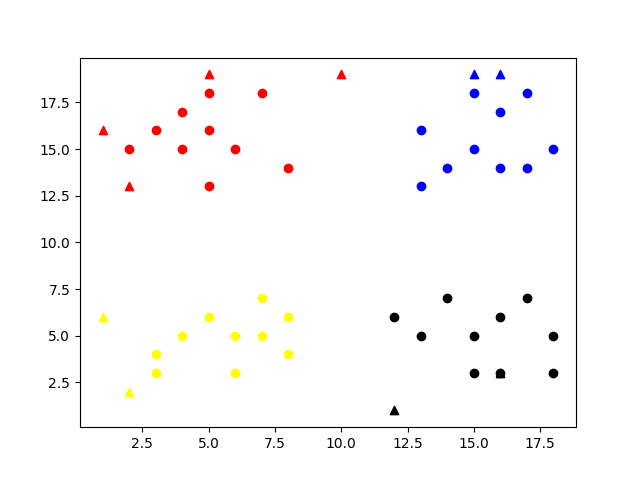
\includegraphics[width=0.8\textwidth]{miniknn.png}
  \caption{Visualization of KNN classification results on 2D data.}
  \label{fig:miniknn}
\end{figure}

\subsection*{Source Code}
\lstinputlisting[language=Python, caption=miniknn.py]{../miniknn.py}

\vspace{0.5cm}
\hrule
\vspace{0.5cm}

% ==========================================
% PROBLEM 3
% ==========================================
\section*{Problem 3: KNN for Handwriting Recognition (MNIST)}

\textbf{Task:} Implement KNN in \texttt{knn.py} to classify MNIST digits.

The KNN classifier was implemented to classify MNIST digits using Euclidean distance. The algorithm was tested on the first 20 images of the test set with $K=10$. The implementation achieved a classification accuracy of $1.0$ (100\%) on this subset. The execution time was approximately 3 seconds.

\subsection*{Source Code}
\lstinputlisting[language=Python, caption=knn.py]{../knn.py}

\subsection*{Execution Output}
\begin{verbatim}
---classification accuracy for knn on mnist: 1.0 ---
---execution time: 2.954530954360962 seconds ---
\end{verbatim}

\end{document}